\documentclass[12pt,a4paper]{article}
\usepackage[utf8]{inputenc}
\usepackage[T2A]{fontenc}
\usepackage[ukrainian]{babel}
\usepackage{geometry}
\usepackage{amsmath}
\usepackage{amssymb}
\usepackage{booktabs}
\usepackage{float}
\usepackage{graphicx}

\geometry{left=2cm, right=2cm, top=2cm, bottom=2cm}

\begin{document}

\begin{center}
{\Large \textbf{Лабораторна робота 5}}\\[0.2cm]
\textbf{Розпізнавання образів, VAR 3 (N=2)}
\end{center}

\section*{Вихідні дані}
У роботі згенеровано три класи в $\mathbb{R}^3$ по 120 навчальних і 120 тестових точок у кожному класі.
Навчальні дані створювались рівномірно по координатах за фіксованим seed $42$.

\section*{Мета}
Побудувати класифікатор для трьох 3D-класів через проєкцію на кандидатні прямі між центрами класів та порівняти дві оцінки вибору прямої.

\section*{Постановка і критерії}
Кандидатні прямі: $L_{12}$, $L_{23}$, $L_{13}$ (між центрами класів).

Для точки $x$ проєкція на пряму $L$:
\[
t(x)=(x-o)^\top u.
\]

У ноутбуці \texttt{lab5/lab-5.ipynb} використано два критерії:
\begin{enumerate}
    \item \textbf{sum\_dist} (мінімізувати): сума ортогональних відстаней усіх навчальних точок до прямої.
    \item \textbf{proj\_msd} (максимізувати): середньоквадратична попарна відстань між усіма 1D-проєкціями точок на пряму.
\end{enumerate}

Для точки $x$ проєкція на пряму $L$ обчислюється як
\[
t(x)=(x-o)^\top u,
\]
де $o$ --- точка на прямій, а $u$ --- одиничний напрямний вектор.

\section*{Результати вибору прямої}
\begin{table}[H]
\centering
\begin{tabular}{lrrr}
\toprule
\textbf{Пряма} & \textbf{sum\_dist} & \textbf{mean\_dist} & \textbf{proj\_msd} \\
\midrule
Клас 1 -- Клас 2 & 1639.3456 & 4.5537 & 31.0353 \\
Клас 2 -- Клас 3 & 1560.6149 & 4.3350 & 35.2145 \\
Клас 1 -- Клас 3 & 1373.2384 & 3.8146 & 44.5884 \\
\bottomrule
\end{tabular}
\end{table}

Найкраща пряма за обома критеріями: \textbf{Клас 1 -- Клас 3}.

У поточній реалізації для класифікації використовується саме ця пряма. Для неї класова структура на проєкції найбільш роздільна, а сумарна відстань точок до прямої мінімальна.

\section*{Скріншоти з ноутбука}
Нижче наведено дві візуалізації, згенеровані з ноутбука: 3D-проєкцію точок на обрану пряму та їх 1D-проєкції на цю ж пряму.

\begin{figure}[H]
\centering
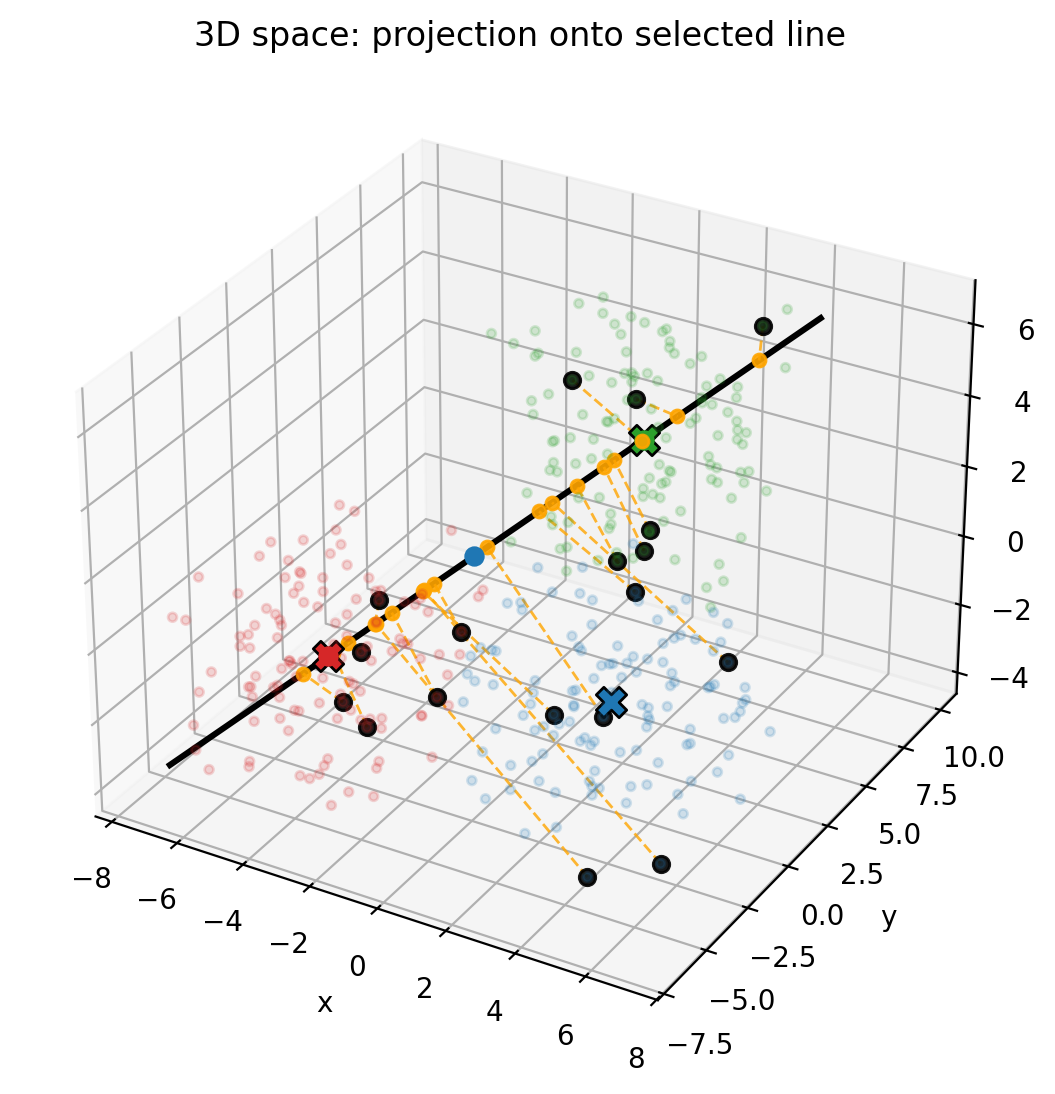
\includegraphics[width=0.95\textwidth]{figures/lab5_3d.png}
\caption{Скріншот з ноутбука: 3D-проєкція навчальних і тестових точок на обрану пряму}
\end{figure}

\begin{figure}[H]
\centering
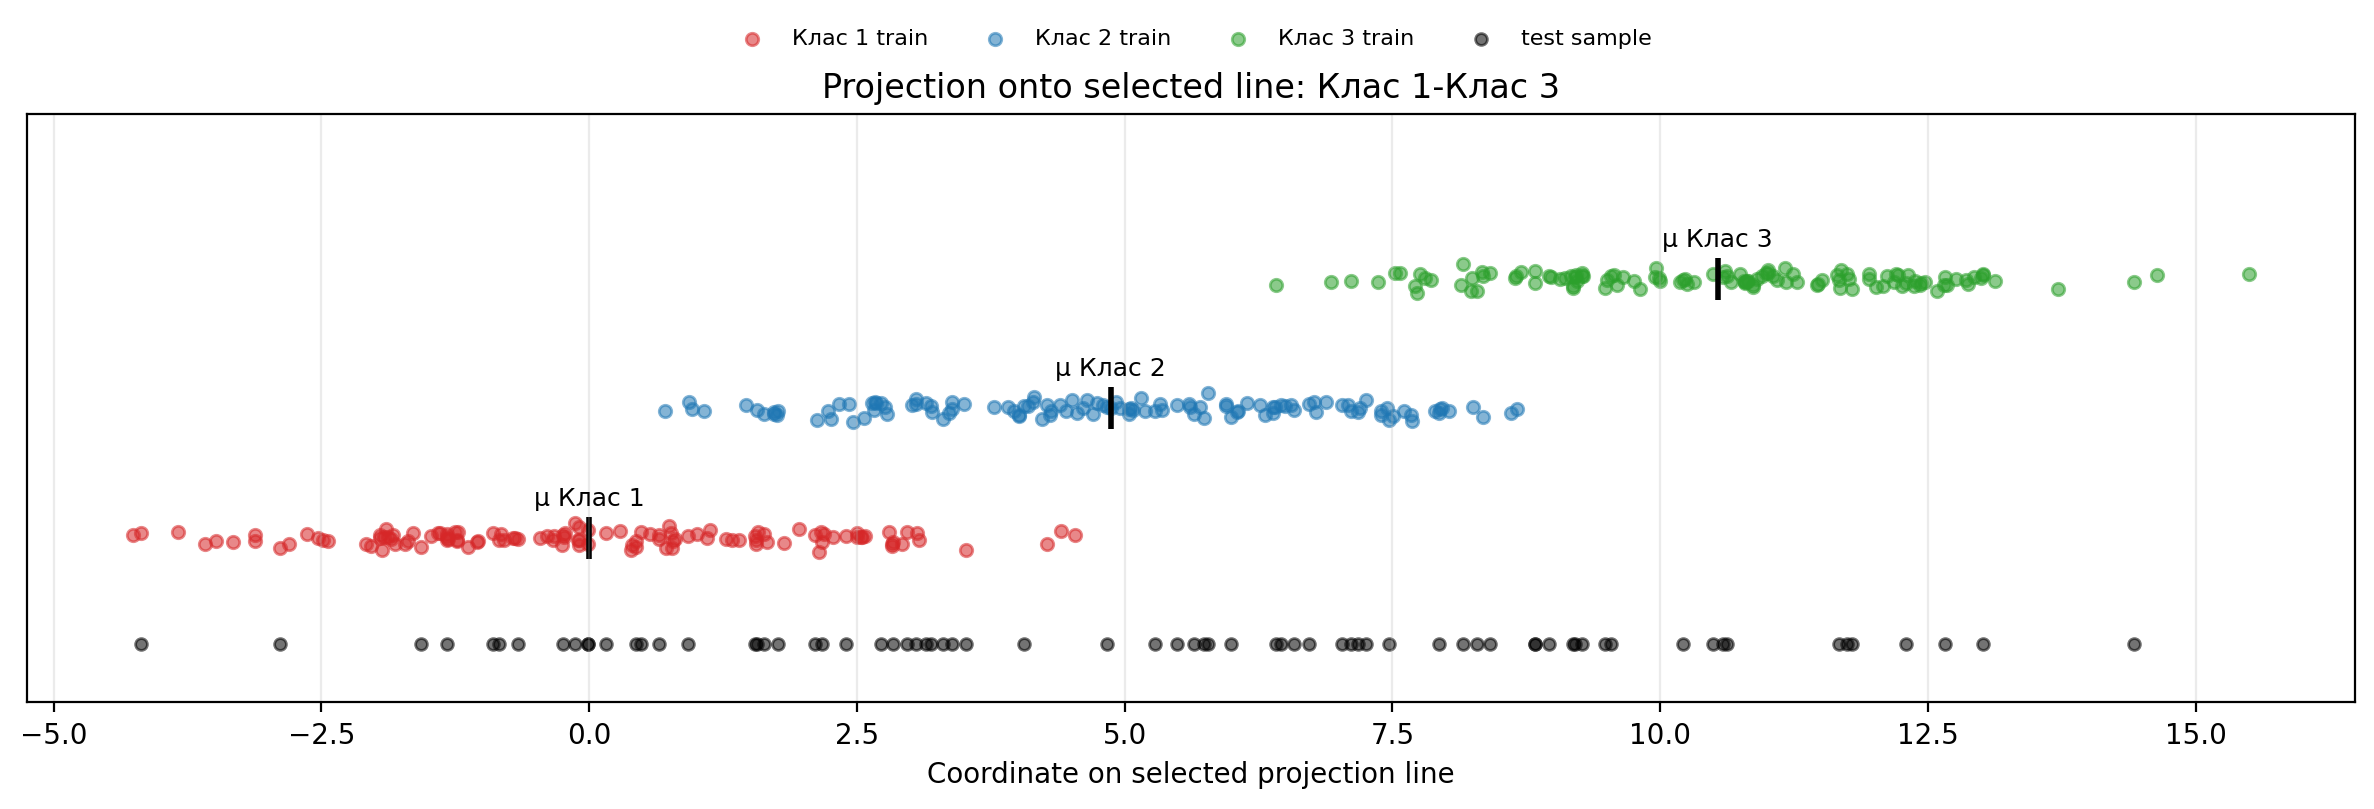
\includegraphics[width=0.95\textwidth]{figures/lab5_1d.png}
\caption{Скріншот з ноутбука: 1D-проєкція точок на обрану пряму}
\end{figure}

\section*{Класифікація}
Рішення для тестової точки приймається за найближчою проєкцією центру класу на обрану пряму:
\[
\hat y(x)=\arg\min_k |t(x)-t(\mu_k)|.
\]

Підсумкова точність на тесті: \textbf{Accuracy = 0.8639}.

На тестовій вибірці модель краще за все відділяє класи саме після проєкції на пряму Клас 1 -- Клас 3.

\section*{Висновок}
Для цієї вибірки пряма Клас 1 -- Клас 3 є найкращою одночасно за критерієм близькості точок до прямої (sum\_dist) і за критерієм розкиду проєкцій (proj\_msd). Класифікація за проєкцією центрів дала точність 0.8639, що підтверджує працездатність обраної схеми.

\end{document}
